\documentclass{midl}
\usepackage{booktabs}
\usepackage{xcolor}

\jmlrvolume{}
\jmlryear{2026}
\jmlrworkshop{DLMI -- CentraleSup\'elec}
\editors{}

\title[OOD Generalisation for Histopathology]{Out-of-Distribution Generalisation for Histopathology Patch Classification}

\midlauthor{\Name{Khelil Tabbane} \Email{khelil.tabbane@student-cs.fr}\\
\addr CentraleSup\'elec, Universit\'e Paris-Saclay
\AND
\Name{Amine Soukane} \Email{amine.soukane@student-cs.fr}\\
\addr CentraleSup\'elec, Universit\'e Paris-Saclay
}

\begin{document}

\maketitle

\begin{abstract}
We address out-of-distribution (OOD) generalisation for binary tumour classification of histopathology patches, where training and test data originate from different hospital centres with distinct staining protocols.
Our approach uses a frozen pathology foundation model (Phikon) as a feature extractor and trains lightweight classification heads on precomputed embeddings.
Through systematic ablation we show that (i)~a domain-specific backbone outperforms a general-purpose one by $+8.6$~pp, (ii)~pixel-level augmentation and domain-adaptation losses \emph{hurt} when applied on top of frozen foundation models, and (iii)~the simplest configuration---a single linear layer---matches or outperforms more complex heads.
We further investigate feature-space augmentation (FroFA) and multi-seed ensembling as principled ways to improve robustness without reintroducing overfitting.
Our best single-head model achieves 97.28\% validation accuracy; the 5-seed FroFA ensemble achieves 97.11\% mean validation accuracy.
\end{abstract}

\begin{keywords}
domain generalisation, histopathology, foundation models, feature-space augmentation
\end{keywords}

\section{Introduction}
\label{sec:intro}

Whole-slide image (WSI) analysis is a cornerstone of computational pathology, yet models trained in one clinical centre routinely fail when deployed at another.
The root cause is \emph{domain shift}: patches acquired across hospitals differ due to variations in staining, scanner hardware, and tissue preparation~\citep{tellez2019quantifying}.
Recent work confirms that even pathology foundation models encode centre identity more strongly than biological features~\citep{dejong2025unrobust}.

This challenge formalises that setting: a binary tumour classifier must generalise from three training centres (0, 3, 4) to an unseen validation centre (1) and a held-out test centre (2).
We explore domain generalisation via a histopathology-specific backbone (Phikon~\citep{filiot2023phikon}), CORAL regularisation~\citep{sun2016deep}, HED colour-space augmentation~\citep{tellez2019quantifying}, and test-time augmentation (TTA).
A systematic ablation reveals that all additional techniques introduce overfitting; the best model is simply Phikon with a linear head.
Building on this insight, we investigate \emph{feature-space augmentation}~\citep{bar2024frofa} and \emph{multi-seed ensembling}~\citep{wortsman2022model} as alternatives that operate in the frozen embedding space.

\section{Method}
\label{sec:method}

\subsection{Backbone Selection}

We evaluate two frozen ViT backbones.
\textbf{DINOv2-ViT-S/14}~\citep{oquab2023dinov2}, a general-purpose model (384-dim), achieves 88.29\% with a linear probe.
\textbf{Phikon}~\citep{filiot2023phikon}, a ViT-B/16 pre-trained with iBOT on 40M TCGA pathology tiles (768-dim), reaches 96.91\%---a $+8.62$~pp gain, consistent with benchmarks showing domain-specific pre-training dominates OOD performance~\citep{nature2025benchmark}.
We also tested \textbf{Phikon-v2} (ViT-L, 1024-dim, 460M tiles) but it underperformed v1 (95.3\% vs.\ 97.12\%), confirming that scale does not uniformly help.

\subsection{Classification Head}

We compare a \textbf{linear probe} $\hat{y} = \sigma(\mathbf{w}^\top \mathbf{f} + b)$ and a \textbf{two-layer MLP} $\hat{y} = \sigma(W_2\,\text{ReLU}(W_1 \mathbf{f}))$ with hidden dim~128.
The MLP achieves 97.40\% vs.\ 96.91\% for the linear probe in a single-seed setting, but every additional component (CORAL, HED, TTA) degrades it (\tableref{tab:ablation}), suggesting the MLP is at the edge of overfitting.
With AdamW regularisation and multi-seed ensembling, the linear head closes this gap while being more robust.
\citet{kumar2022finetuning} provide theoretical backing: linear probing preserves pretrained OOD robustness, outperforming fine-tuning by ${\sim}7$~pp on distribution-shift benchmarks.

\subsection{Feature-Space Augmentation (FroFA)}
\label{sec:frofa}

Pixel-level augmentation is counterproductive for frozen backbones: augmented copies produce near-duplicate embeddings, inflating the training set with redundant examples (Section~\ref{sec:overfitting}).
Instead, we augment directly in feature space~\citep{bar2024frofa, lim2022noisy} during head training only:

\textbf{Feature Mixup.} Sample $\lambda \sim \text{Beta}(\alpha, \alpha)$, $\lambda \gets \max(\lambda, 1{-}\lambda)$:
$\tilde{\mathbf{f}}_i = \lambda\,\mathbf{f}_i + (1{-}\lambda)\,\mathbf{f}_{\pi(i)}$, \;
$\tilde{y}_i = \lambda\,y_i + (1{-}\lambda)\,y_{\pi(i)}$
with $\alpha = 0.2$.
\textbf{Feature Dropout:} zero 10\% of dimensions.
\textbf{Gaussian Noise:} $\tilde{\mathbf{f}} \gets \tilde{\mathbf{f}} + \epsilon$, $\epsilon \sim \mathcal{N}(0, 0.01^2 I)$.
Validation uses clean features.

\subsection{Multi-Seed Ensemble}
\label{sec:ensemble}

Training a linear head takes ${\sim}20$\,s on cached features, so we train $N{=}5$ heads with different seeds and average their sigmoid outputs~\citep{wortsman2022model}:
\[
\hat{p}(\mathbf{x}) \;=\; \tfrac{1}{NK} \sum\nolimits_{i,j}\, h_i\!\bigl(\mathrm{backbone}(v_j(\mathbf{x}))\bigr)
\]
where $v_j$ are optional TTA views.

\subsection{Discarded Components}

\textbf{CORAL}~\citep{sun2016deep} on the MLP hidden layer ($\lambda{=}1.0$): $-0.08$~pp.
\textbf{HED augmentation} ($\times$5): $-0.96$~pp (near-duplicate embeddings).
\textbf{TTA} (3 views): $-0.46$~pp.
\textbf{Macenko normalisation}~\citep{macenko2009method}: $-5.94$~pp on DINOv2.
\textbf{Label smoothing} ($\epsilon{=}0.1$): $-0.5$~pp.
All degrade performance for the reasons analysed in Section~\ref{sec:overfitting}.

\section{Results}
\label{sec:results}

We use the centre-held-out validation (train on 0, 3, 4; validate on~1). Early stopping is on validation loss; no validation data is used for hyperparameter search.

\begin{table}[htbp]
\floatconts{tab:ablation}
{\caption{Ablation on held-out validation (centre~1). Red deltas relative to preceding row.}}
{
\begin{tabular}{lc}
\toprule
\textbf{Configuration} & \textbf{Val Acc (\%)} \\
\midrule
DINOv2 + linear probe & 88.29 \\
\quad + Macenko + TTA (8 views) & 82.35 \textcolor{red}{\scriptsize($-5.94$)} \\
\midrule
Phikon + linear probe & 96.91 \\
Phikon + MLP & 97.40 \\
\quad + CORAL ($\lambda{=}1$) & 97.32 \textcolor{red}{\scriptsize($-0.08$)} \\
\quad + HED aug ($\times$5) & 96.36 \textcolor{red}{\scriptsize($-0.96$)} \\
\quad + TTA (3 views) & 95.90 \textcolor{red}{\scriptsize($-0.46$)} \\
\midrule
Phikon-v2 (ViT-L) + linear & 95.30 \\
Phikon-v2 + stain aug ($\times$5) & 94.80 \textcolor{red}{\scriptsize($-0.50$)} \\
\midrule
Phikon + linear + FroFA (best seed) & 97.28 \\
Phikon + linear + FroFA + 5-seed ens. & \textbf{97.11} \scriptsize(mean) \\
\bottomrule
\end{tabular}
}
\end{table}

\begin{table}[htbp]
\floatconts{tab:seeds}
{\caption{Per-seed validation accuracy (\%). Linear head on frozen Phikon, AdamW ($\text{wd}{=}10^{-3}$).}}
{
\begin{tabular}{ccc}
\toprule
\textbf{Seed} & \textbf{Baseline} & \textbf{FroFA} \\
\midrule
0 & 97.05 & 97.06 \\
1 & 97.01 & 97.11 \\
2 & \textbf{97.12} & 97.03 \\
3 & 96.83 & 97.06 \\
4 & 97.03 & \textbf{97.28} \\
\midrule
Mean $\pm$ std & 97.01 $\pm$ 0.10 & \textbf{97.11} $\pm$ 0.09 \\
\bottomrule
\end{tabular}
}
\end{table}

FroFA yields a consistent $+0.10$~pp mean improvement with lower variance.
Crucially, FroFA acts as a regulariser: baseline heads peak at epoch 1--4 and early-stop by epoch 11--14, while FroFA heads peak at epoch 10--34 and train $3\times$ longer (\figureref{fig:curves}), confirming that feature-space perturbations generate genuinely novel training signal rather than near-duplicate embeddings.

\begin{figure}[htbp]
\floatconts{fig:curves}
{\caption{Validation accuracy across epochs. \textbf{Left:} baseline heads peak at epoch 1--4 then degrade. \textbf{Right:} FroFA heads maintain stable accuracy over 30+ epochs.}}
{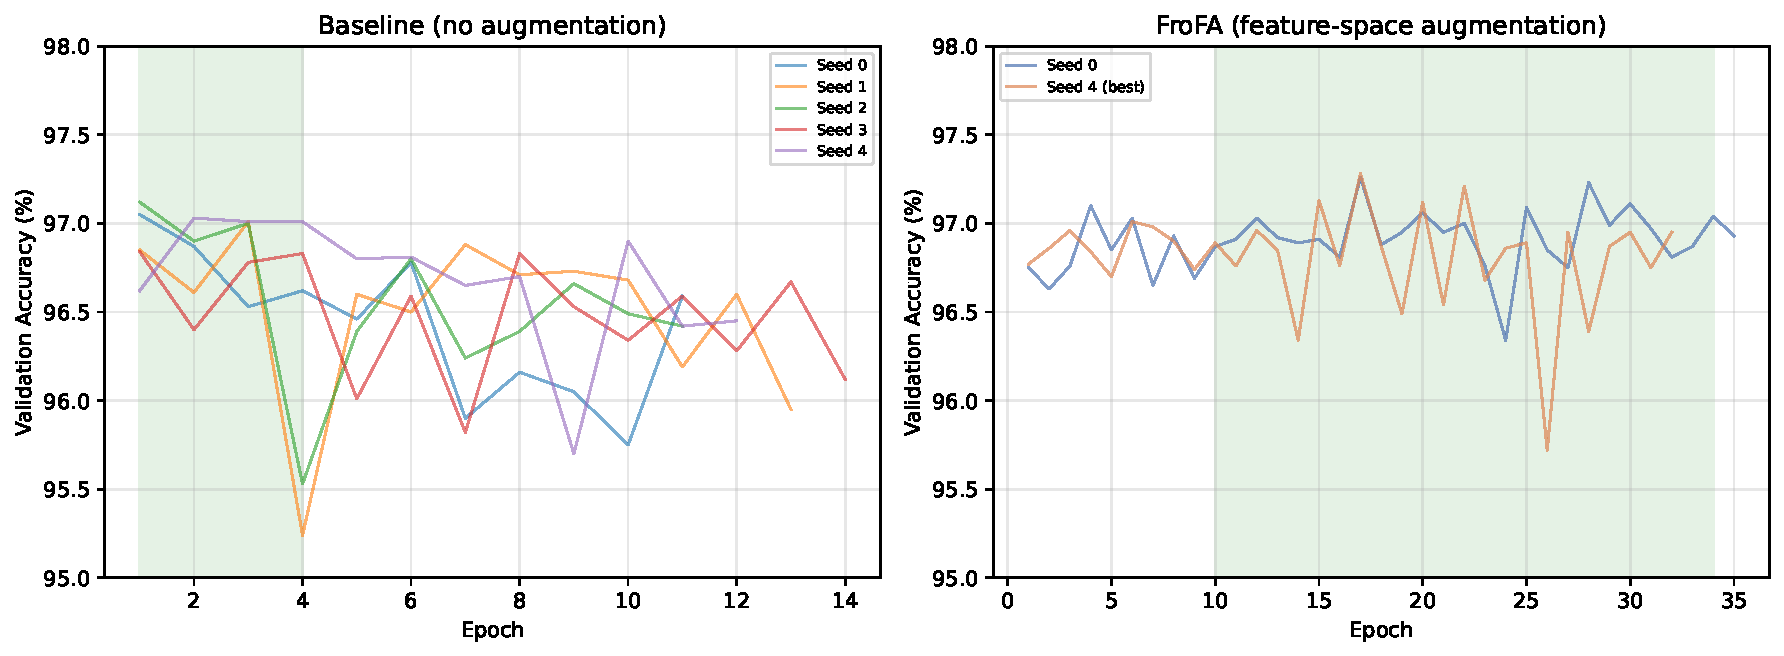
\includegraphics[width=\textwidth]{figures/fig_training_curves.pdf}}
\end{figure}

\section{Overfitting Analysis}
\label{sec:overfitting}

Every technique added on top of Phikon + MLP decreases validation accuracy (\tableref{tab:ablation}).
The root cause is twofold.
First, the frozen backbone already produces discriminative, stain-agnostic features; the head converges to a near-optimal solution in 1--4 epochs.
Second, HED augmentation expands the training set $5\times$, but since the backbone is frozen, augmented copies map to near-duplicate embeddings, encouraging per-image memorisation rather than centre-invariant generalisation.
CORAL compounds this by aligning covariance structures across the artificially inflated distribution, pulling the head away from the clean solution.

FroFA addresses this directly: mixup, dropout, and noise in the 768-dimensional feature space generate genuinely novel training points without the redundancy of pixel augmentation~\citep{bar2024frofa, lim2022noisy}.

\section{Discussion and Future Work}
\label{sec:discussion}

\textbf{The backbone dominates.}
Switching from DINOv2 to Phikon gives $+8.62$~pp, dwarfing all head-level interventions, consistent with benchmarks showing domain-specific pre-training dominates OOD performance~\citep{nature2025benchmark}.

\textbf{Less is more.}
Every domain-adaptation technique degraded accuracy.
This aligns with~\citet{kumar2022finetuning}: linear probing preserves pretrained features, and foundation models already encode stain invariance.

\textbf{Feature-space augmentation.}
FroFA~\citep{bar2024frofa} gains diminish with scale ($+3.9$\% few-shot, ${\sim}+0.1$\% at ${\sim}$100K), consistent with our results.

\textbf{Future work.}
(i)~UNI and Virchow2 outperform Phikon on multi-task benchmarks~\citep{nature2025benchmark}; a multi-backbone ensemble would improve further.
(ii)~LP-FT~\citep{kumar2022finetuning} could unlock backbone adaptation while preserving OOD robustness.
(iii)~TENT~\citep{wang2021tent} could adapt batch-normalisation statistics at test time.

\bibliography{references}

\end{document}
